\makeatletter\def\fps@figure{tp}\makeatother\renewcommand{\topfraction}{0.9}\renewcommand{\textfraction}{0.1}

\begin{figure}
\centering
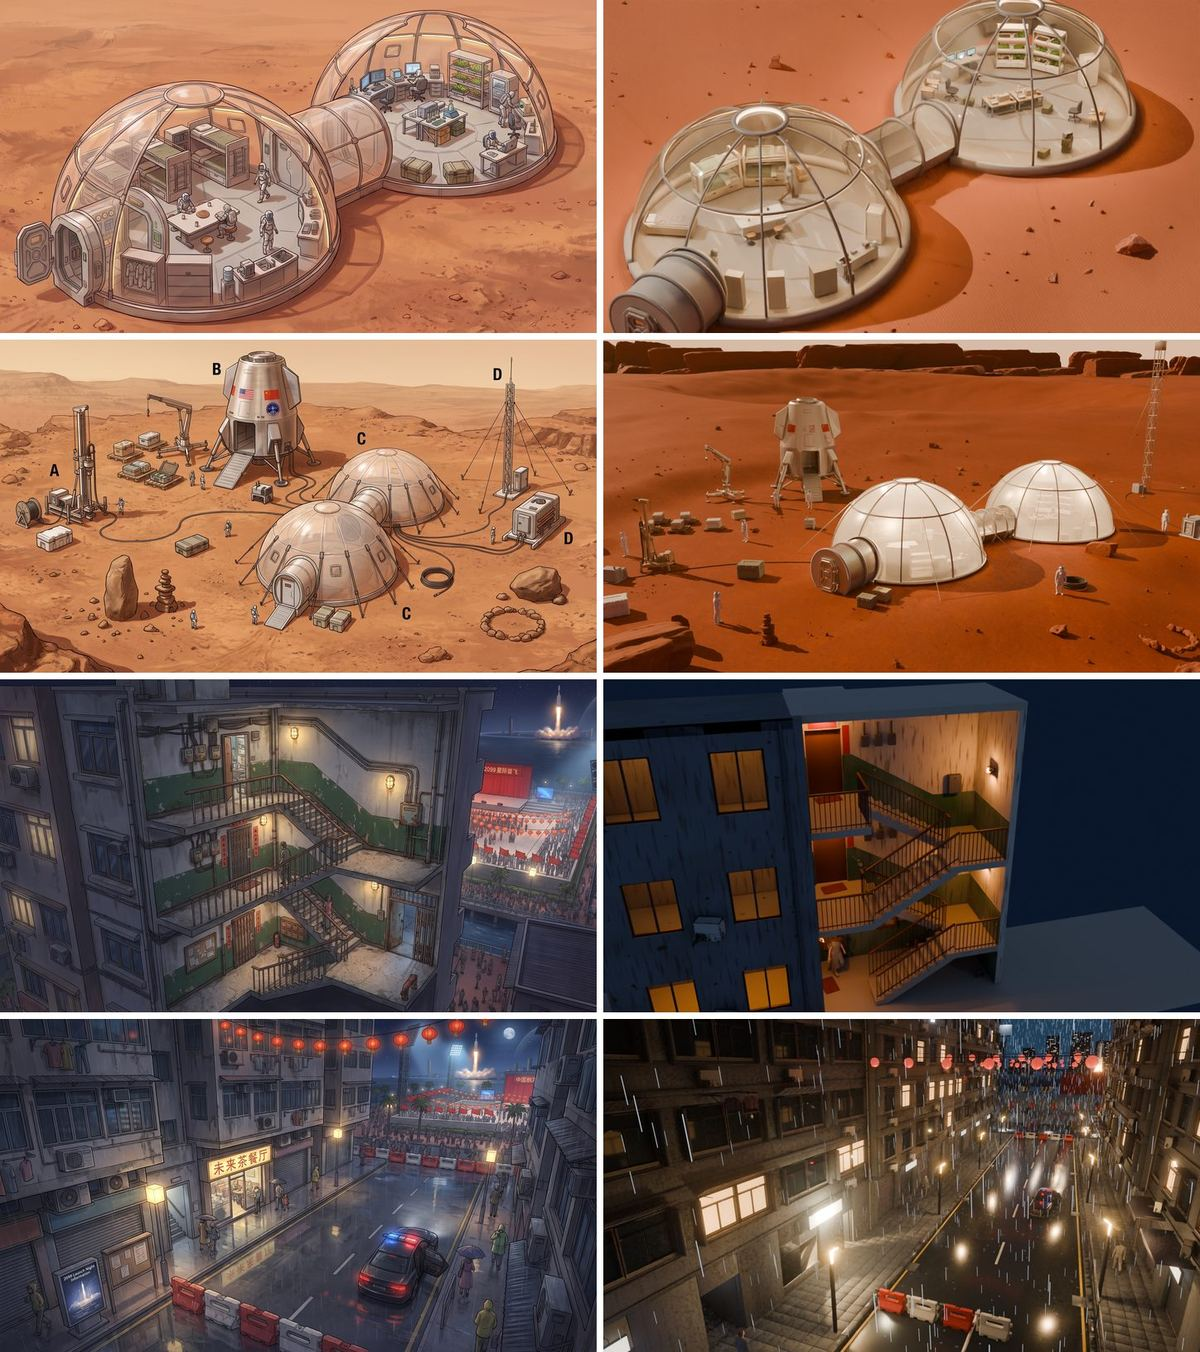
\includegraphics[width=1\linewidth,height=\textheight,keepaspectratio,alt={Each place's locked concept (left) beside the final render of its scene from the concept's own view (right): camp, campgrounds, stairwell and street, top to bottom. Every object in the renders is a library entry laid by the placing agent, and every scene passes the physics-readiness check with no fault.}]{figures/places.jpg}
\caption{Each place's locked concept (left) beside the final render of its scene from the concept's own view (right): camp, campgrounds, stairwell and street, top to bottom. Every object in the renders is a library entry laid by the placing agent, and every scene passes the physics-readiness check with no fault.}
\end{figure}
